
%% bare_conf.tex
%% V1.4
%% 2012/12/27
%% by Michael Shell
%% See:
%% http://www.michaelshell.org/
%% for current contact information.
%%
%% This is a skeleton file demonstrating the use of IEEEtran.cls
%% (requires IEEEtran.cls version 1.8 or later) with an IEEE conference paper.
%%
%% Support sites:
%% http://www.michaelshell.org/tex/ieeetran/
%% http://www.ctan.org/tex-archive/macros/latex/contrib/IEEEtran/
%% and
%% http://www.ieee.org/

\documentclass[conference]{IEEEtran}
% Add the compsoc option for Computer Society conferences.
%
% If IEEEtran.cls has not been installed into the LaTeX system files,
% manually specify the path to it like:
% \documentclass[conference]{../sty/IEEEtran}


% *** MISC UTILITY PACKAGES ***
%
%\usepackage{ifpdf}
% Heiko Oberdiek's ifpdf.sty is very useful if you need conditional
% compilation based on whether the output is pdf or dvi.
% usage:
% \ifpdf
%   % pdf code
% \else
%   % dvi code
% \fi
% The latest version of ifpdf.sty can be obtained from:
% http://www.ctan.org/tex-archive/macros/latex/contrib/oberdiek/
% Also, note that IEEEtran.cls V1.7 and later provides a builtin
% \ifCLASSINFOpdf conditional that works the same way.
% When switching from latex to pdflatex and vice-versa, the compiler may
% have to be run twice to clear warning/error messages.


% *** CITATION PACKAGES ***
%
%\usepackage{cite}
% cite.sty was written by Donald Arseneau
% V1.6 and later of IEEEtran pre-defines the format of the cite.sty package
% \cite{} output to follow that of IEEE. Loading the cite package will
% result in citation numbers being automatically sorted and properly
% "compressed/ranged". e.g., [1], [9], [2], [7], [5], [6] without using
% cite.sty will become [1], [2], [5]--[7], [9] using cite.sty. cite.sty's
% \cite will automatically add leading space, if needed. Use cite.sty's
% noadjust option (cite.sty V3.8 and later) if you want to turn this off
% such as if a citation ever needs to be enclosed in parenthesis.
% cite.sty is already installed on most LaTeX systems. Be sure and use
% version 4.0 (2003-05-27) and later if using hyperref.sty. cite.sty does
% not currently provide for hyperlinked citations.
% The latest version can be obtained at:
% http://www.ctan.org/tex-archive/macros/latex/contrib/cite/
% The documentation is contained in the cite.sty file itself.




\usepackage{graphicx}
\graphicspath{{./images/}}

% *** GRAPHICS RELATED PACKAGES ***
%
\ifCLASSINFOpdf
  % \usepackage[pdftex]{graphicx}
  % declare the path(s) where your graphic files are
  % \graphicspath{{../pdf/}{../jpeg/}}
  % and their extensions so you won't have to specify these with
  % every instance of \includegraphics
  % \DeclareGraphicsExtensions{.pdf,.jpeg,.png}
\else
  % or other class option (dvipsone, dvipdf, if not using dvips). graphicx
  % will default to the driver specified in the system graphics.cfg if no
  % driver is specified.
  % \usepackage[dvips]{graphicx}
  % declare the path(s) where your graphic files are
  % \graphicspath{{../eps/}}
  % and their extensions so you won't have to specify these with
  % every instance of \includegraphics
  % \DeclareGraphicsExtensions{.eps}
\fi
% graphicx was written by David Carlisle and Sebastian Rahtz. It is
% required if you want graphics, photos, etc. graphicx.sty is already
% installed on most LaTeX systems. The latest version and documentation
% can be obtained at: 
% http://www.ctan.org/tex-archive/macros/latex/required/graphics/
% Another good source of documentation is "Using Imported Graphics in
% LaTeX2e" by Keith Reckdahl which can be found at:
% http://www.ctan.org/tex-archive/info/epslatex/
%
% latex, and pdflatex in dvi mode, support graphics in encapsulated
% postscript (.eps) format. pdflatex in pdf mode supports graphics
% in .pdf, .jpeg, .png and .mps (metapost) formats. Users should ensure
% that all non-photo figures use a vector format (.eps, .pdf, .mps) and
% not a bitmapped formats (.jpeg, .png). IEEE frowns on bitmapped formats
% which can result in "jaggedy"/blurry rendering of lines and letters as
% well as large increases in file sizes.
%
% You can find documentation about the pdfTeX application at:
% http://www.tug.org/applications/pdftex





% *** MATH PACKAGES ***
%
%\usepackage[cmex10]{amsmath}
% A popular package from the American Mathematical Society that provides
% many useful and powerful commands for dealing with mathematics. If using
% it, be sure to load this package with the cmex10 option to ensure that
% only type 1 fonts will utilized at all point sizes. Without this option,
% it is possible that some math symbols, particularly those within
% footnotes, will be rendered in bitmap form which will result in a
% document that can not be IEEE Xplore compliant!
%
% Also, note that the amsmath package sets \interdisplaylinepenalty to 10000
% thus preventing page breaks from occurring within multiline equations. Use:
%\interdisplaylinepenalty=2500
% after loading amsmath to restore such page breaks as IEEEtran.cls normally
% does. amsmath.sty is already installed on most LaTeX systems. The latest
% version and documentation can be obtained at:
% http://www.ctan.org/tex-archive/macros/latex/required/amslatex/math/





% *** SPECIALIZED LIST PACKAGES ***
%
%\usepackage{algorithmic}
% algorithmic.sty was written by Peter Williams and Rogerio Brito.
% This package provides an algorithmic environment fo describing algorithms.
% You can use the algorithmic environment in-text or within a figure
% environment to provide for a floating algorithm. Do NOT use the algorithm
% floating environment provided by algorithm.sty (by the same authors) or
% algorithm2e.sty (by Christophe Fiorio) as IEEE does not use dedicated
% algorithm float types and packages that provide these will not provide
% correct IEEE style captions. The latest version and documentation of
% algorithmic.sty can be obtained at:
% http://www.ctan.org/tex-archive/macros/latex/contrib/algorithms/
% There is also a support site at:
% http://algorithms.berlios.de/index.html
% Also of interest may be the (relatively newer and more customizable)
% algorithmicx.sty package by Szasz Janos:
% http://www.ctan.org/tex-archive/macros/latex/contrib/algorithmicx/




% *** ALIGNMENT PACKAGES ***
%
%\usepackage{array}
% Frank Mittelbach's and David Carlisle's array.sty patches and improves
% the standard LaTeX2e array and tabular environments to provide better
% appearance and additional user controls. As the default LaTeX2e table
% generation code is lacking to the point of almost being broken with
% respect to the quality of the end results, all users are strongly
% advised to use an enhanced (at the very least that provided by array.sty)
% set of table tools. array.sty is already installed on most systems. The
% latest version and documentation can be obtained at:
% http://www.ctan.org/tex-archive/macros/latex/required/tools/


% IEEEtran contains the IEEEeqnarray family of commands that can be used to
% generate multiline equations as well as matrices, tables, etc., of high
% quality.




% *** SUBFIGURE PACKAGES ***
%\ifCLASSOPTIONcompsoc
%  \usepackage[caption=false,font=normalsize,labelfont=sf,textfont=sf]{subfig}
%\else
%  \usepackage[caption=false,font=footnotesize]{subfig}
%\fi
% subfig.sty, written by Steven Douglas Cochran, is the modern replacement
% for subfigure.sty, the latter of which is no longer maintained and is
% incompatible with some LaTeX packages including fixltx2e. However,
% subfig.sty requires and automatically loads Axel Sommerfeldt's caption.sty
% which will override IEEEtran.cls' handling of captions and this will result
% in non-IEEE style figure/table captions. To prevent this problem, be sure
% and invoke subfig.sty's "caption=false" package option (available since
% subfig.sty version 1.3, 2005/06/28) as this is will preserve IEEEtran.cls
% handling of captions.
% Note that the Computer Society format requires a larger sans serif font
% than the serif footnote size font used in traditional IEEE formatting
% and thus the need to invoke different subfig.sty package options depending
% on whether compsoc mode has been enabled.
%
% The latest version and documentation of subfig.sty can be obtained at:
% http://www.ctan.org/tex-archive/macros/latex/contrib/subfig/




% *** FLOAT PACKAGES ***
%
%\usepackage{fixltx2e}
% fixltx2e, the successor to the earlier fix2col.sty, was written by
% Frank Mittelbach and David Carlisle. This package corrects a few problems
% in the LaTeX2e kernel, the most notable of which is that in current
% LaTeX2e releases, the ordering of single and double column floats is not
% guaranteed to be preserved. Thus, an unpatched LaTeX2e can allow a
% single column figure to be placed prior to an earlier double column
% figure. The latest version and documentation can be found at:
% http://www.ctan.org/tex-archive/macros/latex/base/


%\usepackage{stfloats}
% stfloats.sty was written by Sigitas Tolusis. This package gives LaTeX2e
% the ability to do double column floats at the bottom of the page as well
% as the top. (e.g., "\begin{figure*}[!b]" is not normally possible in
% LaTeX2e). It also provides a command:
%\fnbelowfloat
% to enable the placement of footnotes below bottom floats (the standard
% LaTeX2e kernel puts them above bottom floats). This is an invasive package
% which rewrites many portions of the LaTeX2e float routines. It may not work
% with other packages that modify the LaTeX2e float routines. The latest
% version and documentation can be obtained at:
% http://www.ctan.org/tex-archive/macros/latex/contrib/sttools/
% Do not use the stfloats baselinefloat ability as IEEE does not allow
% \baselineskip to stretch. Authors submitting work to the IEEE should note
% that IEEE rarely uses double column equations and that authors should try
% to avoid such use. Do not be tempted to use the cuted.sty or midfloat.sty
% packages (also by Sigitas Tolusis) as IEEE does not format its papers in
% such ways.
% Do not attempt to use stfloats with fixltx2e as they are incompatible.
% Instead, use Morten Hogholm'a dblfloatfix which combines the features
% of both fixltx2e and stfloats:
%
% \usepackage{dblfloatfix}
% The latest version can be found at:
% http://www.ctan.org/tex-archive/macros/latex/contrib/dblfloatfix/




% *** PDF, URL AND HYPERLINK PACKAGES ***
%
%\usepackage{url}
% url.sty was written by Donald Arseneau. It provides better support for
% handling and breaking URLs. url.sty is already installed on most LaTeX
% systems. The latest version and documentation can be obtained at:
% http://www.ctan.org/tex-archive/macros/latex/contrib/url/
% Basically, \url{my_url_here}.




% *** Do not adjust lengths that control margins, column widths, etc. ***
% *** Do not use packages that alter fonts (such as pslatex).         ***
% There should be no need to do such things with IEEEtran.cls V1.6 and later.
% (Unless specifically asked to do so by the journal or conference you plan
% to submit to, of course. )


% correct bad hyphenation here
\hyphenation{op-tical net-works semi-conduc-tor}
\usepackage{verbatim}
\usepackage{multirow}
\usepackage{tabulary}
\usepackage[labelformat=empty]{caption}
\usepackage{float}
\restylefloat{table}

\usepackage{alltt}
\usepackage{flushend}

\clubpenalty = 10000
\widowpenalty = 10000
\displaywidowpenalty = 10000

\begin{document}
%
% paper title
% can use linebreaks \\ within to get better formatting as desired
% Do not put math or special symbols in the title.

\title{Reassessing the Pattern-based Approach for \\Formalizing Requirements in \\the Automotive Domain}


% author names and affiliations
% use a multiple column layout for up to three different
% affiliations
\author{\IEEEauthorblockN{Predrag Filipovikj}
\IEEEauthorblockA{M\"{a}lardalen University \\
V\"{a}ster{\aa}s, Sweden \\
predrag.filipovikj@mdh.se}
\and
\IEEEauthorblockN{Mattias Nyberg}
\IEEEauthorblockA{Scania\\
S\"{o}dert\"{a}lje, Sweden \\
mattias.nyberg@scania.com}
\and
\IEEEauthorblockN{Guillermo Rodriguez-Navas}
\IEEEauthorblockA{M\"{a}lardalen University \\
V\"{a}ster{\aa}s, Sweden \\
guillermo.rodriguez-navas@mdh.se}
}

% make the title area
\maketitle

% As a general rule, do not put math, special symbols or citations
% in the abstract

\begin{abstract}
The importance of using formal methods and techniques for verification of requirements in the automotive industry has been greatly emphasized with the introduction of the new ISO26262  standard for road vehicles functional safety. The lack of support for formal modeling of requirements still represents an obstacle for the adoption of the formal methods in industry. This paper presents a case study that has been conducted in order to evaluate the difficulties inherent to the process of transforming the system requirements from their traditional written form into semi-formal notation. The case study focuses on a set of non-structured functional requirements for the Electrical and Electronic (E/E) systems inside heavy road vehicles, written in natural language, and reassesses the applicability of the extended Specification Pattern System (SPS) represented in a restricted English grammar. Correlating this experience with former studies, we observe that, as previously claimed, the concept of patterns is likely to be generally applicable for the automotive domain. Additionally, we have identified some potential difficulties in the transformation process, which were not reported by the previous studies and will be used as a basis for further research.
\end{abstract}

\section{Introduction}

New and emerging technologies are being incorporated into vehicles, leading to a significant increase of the number and complexity of the implemented functions. Currently, in industrial settings, manual inspection (peer review) is the most widespread technique for checking the correctness of the systems' specification~\cite{Walia09sysLitReview}. Performing these reviews manually is becoming more difficult as the complexity of the specifications increase. Additionally, the fact that the reviewing peers may be different stakeholders, with different backgrounds and interests, and even working at different companies makes it more difficult to guarantee that the specification was properly understood and validated \cite{Heumesser92experienceInAutomotive}. 

In these conditions, it is clear that having tool support for computer-assisted verification of the specifications would speed up the process and be beneficial. The new ISO26262 standard for functional safety of the road vehicles acknowledges this, by advocating the application of formal verification techniques at each level of system abstraction~\cite{iso26262}. 

One of the main problems in order to introduce formal verification techniques in industry is the lack of formal specifications of the systems. The common practice in the automotive industry nowadays is to specify system requirements in natural language, typically using a general purpose text editor. Requirements written like this are ambiguous, cannot be easily processed by computers and provide limited traceability; they are also most likely to be incomplete and/or inconsistent. The most desirable situation would be to have requirements expressed in some kind of logics, for instance with temporal logics such as LTL \cite{Emerson95temporaland}, CTL \cite{Emerson95temporaland} or TCTL \cite{Alur92phd}. Requirements expressed as such can be subject to different forms of automated analysis, like consistency checks and others.

It is not realistic to believe that automotive engineers will be able to easily express system requirements using formal notations. First of all, automotive engineers are in general very knowledgeable about disciplines like mechanics, hydraulics, electronics, mechatronics, etc., but they are not so skilled in computer science and discrete mathematics. Teaching every engineer how to specify properties with temporal logics would require a great amount of time, and would be too costly to be feasible.
Furthermore, it is not only the engineers who need to understand the requirements. Other stakeholders at different levels of the organization, e.g. customer service or maintenance service, must process the requirements and validate them according to their specific needs~\cite{Hull11reBook}.

Several researchers believe that this gap can be filled with the help of software tools that will assist the engineers in the process of \emph{automated transformation} of requirements from natural language into temporal logics \cite{Cobleigh06userguide} \cite{Konrad05facilitating} \cite{Overmyer01conceptual}. This process is often called \emph{formalization of requirements}. There exist some interesting tools on the market providing this functionality~\cite{Holberg11btc}, but they are not widely accepted.
More research is still needed for understanding how the automated formalization of requirements will fit into the development process of an organization. 

This paper presents a preliminary study that has been conducted in order to gain further understanding of the benefits, limitations and challenges encountered when formalizing requirements in a realistic setup. This study has been performed in collaboration with Scania, one of the leading Swedish truck manufacturers. The goal of the case study is to take a small subset of non-structured functional requirements from the E/E systems written in natural language and formalize them using the approach known as Real Time Specification Patterns, developed by Konrad and Cheng \cite{Konrad05sps}. These patterns are based on the set of Specification Pattern System (SPS), initially defined by Dwyer et al. \cite{Dwyer99sps}, but are enriched with patterns that can capture the timing aspect in the requirements. The work by Konrad and Cheng also proposed a system of restricted English grammar, through which the requirements can be expressed in specification patterns more naturally from a linguistic point of view. These patterns have been applied at least in one case study in the automotive domain~\cite{Post12bosch}. A significant advantage of this approach is that each pattern maps into temporal logics, which makes the transition from the restricted English into formal notation automated. This paper summarizes the knowledge gained from this case study, with special emphasis on the challenges faced during the process, and reports future directions for research.

\begin{table*}[hbtp]
\footnotesize
\renewcommand{\arraystretch}{1.3}
\caption {\textbf{Table 1:} Restricted English grammar patterns \cite{Konrad05sps}.} \label{tab:patterns} 
  \begin{center}
    \begin{tabulary}{1.0\textwidth}{| p{0.08\textwidth} | p{0.18\textwidth} p{0.66\textwidth} |}
    \cline{2-3}
    \hline
    \textbf{Start} & property & \textit{scope~“,~”~specification~“.”} \\
    \hline
    \textbf{Scope} & scope & \textit{“Globally”~\textbar~“Before”~R~\textbar~“After”~Q~\textbar~“Between”~Q~“and”~R~\textbar~“After”~Q~“until”~R} \\
    \hline
    \textbf{General} & specification & \textit{qualitativeType~\textbar~realtimeType} \\
    \hline      
\multirow{13}{*}{\textbf{Qualitative}} & qualitativeType & \textit{occurrenceCategory~\textbar~orderCategory} \\
&  occurrenceCategory & \textit{absencePattern~\textbar~universalityPattern~\textbar~existencePattern~\textbar~boundedExistencePattern} \\
  &  absencePattern & \textit{“it is never the case that ”~P~“~holds”} \\
   &  universalityPattern & \textit{“it is always the case that ”~P~“ holds”} \\
    &  existencePattern & \textit{P “eventually holds”} \\
     &  boundedExistencePattern & \textit{“transitions to states in which ” P “ holds occur at most twice”} \\
      &  orderCategory & \textit{“it is always the case that if ”~P~“ holds” (precedencePattern~\textbar~precedenceChainPattern1-2~\textbar~precedenceChainPattern2-1~\textbar~responsePattern~\textbar~responseChainPattern1-2~\textbar~responseChainPattern2-1~\textbar~constrainedChainPattern1-2)} \\
       &  precedencePattern & \textit{“, then ” S “ previously held”} \\
        &  precedenceChainPattern1-2 & \textit{“ and is succeeded by ” S “, then ” T “ previously held”} \\
         &  precedenceChainPattern2-1 & \textit{“, then ” S “ previously held and was preceded by ” T} \\
          &  responsePattern & \textit{“, then ” S “ eventually holds”} \\
           & responseChainPattern1-2 & \textit{“, then ” S “ eventually holds and is succeeded by ” T} \\
            & responseChainPattern2-1 & \textit{“ and is succeeded by ” S “, then ” T “ eventually holds after ” S} \\
            & constrainedChainPattern1-2 & \textit{“, then ” S “ eventually holds and is succeeded by ” T “, where ”
Z “ does not hold between ” S “ and ” T} \\
            \hline
      \multirow{9}{*}{\textbf{Real-time}} & realtimeType & \textit{“it is always the case that ” (durationCategory~\textbar~periodicCategory~\textbar~realtimeOrderCategory )} \\
     
      & durationCategory & \textit{“once ” P “ becomes satisfied, it holds for ” (minDurationPattern~\textbar~maxDurationPattern )} \\
      & minDurationPattern & \textit{“at least ” c “ time unit(s)”} \\
      & maxDurationPattern & \textit{“less than ” c “ time unit(s)”} \\
      & periodicCategory & \textit{P “ holds ” boundedRecurrencePattern} \\
      & boundedRecurrencePattern & \textit{“at least every ” c “ time unit(s)”} \\
      & realtimeOrderCategory & \textit{“if ”~P~“ holds, then ”~S~“~holds~” (boundedResponsePattern~\textbar~boundedInvariancePattern)} \\
      & boundedResponsePattern & \textit{“after at most ” c “ time unit(s)”} \\
      & boundedInvariancePattern & \textit{“for at least ” c “ time unit(s)”} \\
      \hline
    \end{tabulary}
  \end{center}
\end{table*}

\section{Description and setup of the case study}

As already indicated, Post et al. successfully applied Real Time Specification Patterns in a case study within the automotive domain~\cite{Post12bosch}. Our case study is inspired by that experience but also presents some differences. It is similar in the sense that a set of industrial non-structured requirements will be taken and converted into patterns; we will call this process \emph{patterning} of the requirements. But it differs in the way the requirements are gathered and filtered before the patterning happens.

\subsection{Real Time Specification Patterns}

In our case study we use the Real Time Specification Pattern System (RTSP) as defined by Konrad and Cheng \cite{Konrad05sps}. This set of patterns has been chosen because it provides a quantitative notion of time, which is needed for formalization of the real-time requirements. Table 1 shows these patterns together with their representation in restricted English grammar; the list contains 17 specification patterns.
All these patterns share the characteristics of being non-recursive and prone to an automated transformation into temporal logics such as LTL, CTL and TCTL. One should notice that there is no direct mapping of \textit{each} pattern from the RTSP into \textit{every} temporal logics, as there can be patterns with semantics that cannot be expressed in some of the previously mentioned formal notations.

\begin{figure}
  \centering
    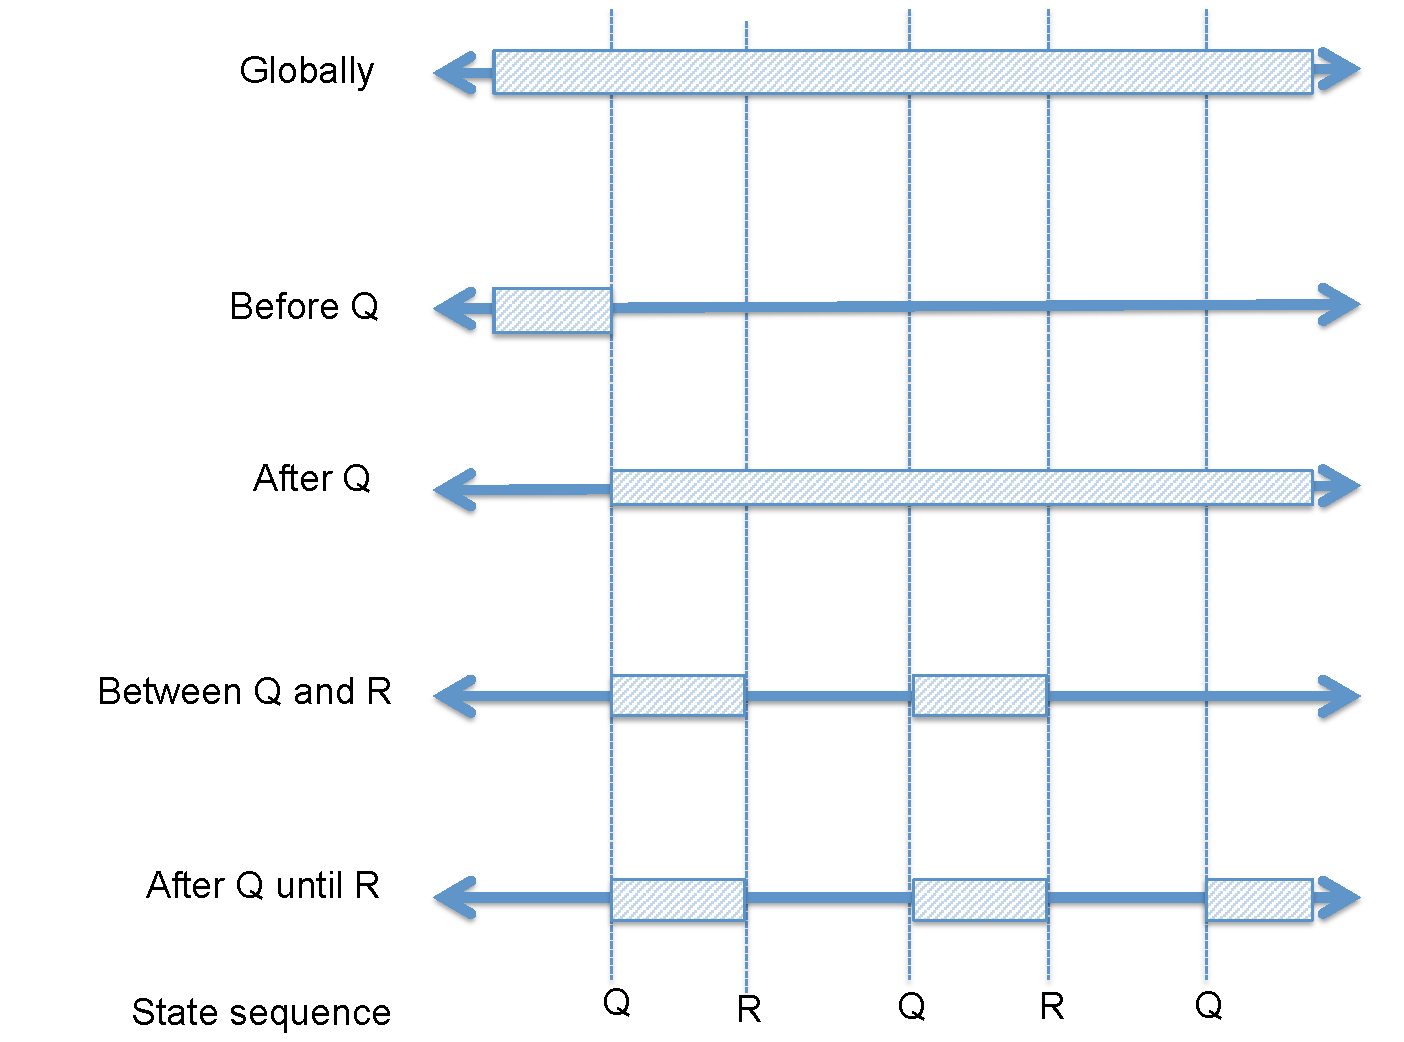
\includegraphics[width=0.47\textwidth]{pattern_scopes_corrected.pdf}
      \caption{\textbf{Figure \ref{fig:patternScopes}:} Pattern scopes \cite{Post12bosch}.}
      \label{fig:patternScopes}
\end{figure}

Each pattern is constituted by literal and non-literal terminals. The non-literal terminals can be either boolean expressions describing system properties, or integer values capturing timing aspects. The remaining parts of the pattern are the literal terminals, which cannot be changed. For example in the \textit{Precedence pattern} given as: ``it is always the case that if \textit{P} holds, then \textit{S} previously held", \textit{P} and \textit{S} represent non-literal terminals and the remaining of the pattern are literal terminals.\\
For each pattern an extent of program execution for which the requirement holds must be defined. As defined by Dwyer et al. \cite{Dwyer99sps}, there are five scopes of program execution: \textit{Globally} (the entire program execution), \textit{Before Q} (until the first occurrence of the state/event Q), \textit{After Q} (after the occurrence of the state/event Q), \textit{Between Q and R} (any part of the program execution between the two states/events Q and R) and After Q until R (similar behavior as Between scope except that the execution continues even if the second state/event never occurs). The graphical representation of the scopes is given in Figure \ref{fig:patternScopes}.


\subsection{Requirements gathering}

In order to collect the requirements for the study, some engineers from Scania were contacted and asked to send requirements documents exemplifying their usual work. In response, we received four documents with a number of non-structured functional requirements written in natural language. Three of the documents were written as MS Word documents, and the other one was written in DOORS.
In total, one hundred requirements were gathered. Although this number is small compared to the total number of requirements of a system, the gathered data was representative enough for the first evaluation of the patterning process.

Regarding the contents, one of the documents included requirements relative to user functions, or UFR in Scania terminology, whereas the other three contained requirements describing the behavior at the sub-system level, known as Allocation Element Requirements (AER) in Scania terminology.

After this gathering, the chosen requirements were extracted from the documents and stored in a data sheet, disposing any other information. This guarantees that only the statements marked as requirements are assessed, and not context information or other meta-data related to them. This gives an indirect measure of the quality of the requirement with respect to automated transformation: if a requirement cannot be patterned without knowing other information appearing in the document, it will most likely not be prone to an automated formalization.

A difference with respect to the previous case study is that the requirements were extracted from the documents by the researchers (not by the engineers) as they were provided, specifically without any filtering or preprocessing. In contrast, Post et al.~\cite{Post12bosch} only considered behavioral requirements, and were preprocessed before the formalization. We proceed differently, because our goal is to investigate to what extent the considered specification patterns can help the verification effort. Since engineers have to verify all kinds of requirements, behavioral and not behavioral, and their starting point is typically the existing documentation, we preferred to stay as close as possible to those conditions.

\subsection{Requirements patterning}

The patterning of the requirements was performed sequentially, one by one, by accessing only the information available in the data sheet. It was preceded by a phase in which the researchers studied the specification patterns and prepared a list
containing all the patterns described in \cite{Post12bosch}, which would be consulted during the process. None of the researchers involved in the process had previous experience with the specification patterns. 

The patterning process consisted in the following tasks: i) identifying which pattern should be applied to the requirement and after that, ii) writing the requirement in restricted English grammar according to the chosen pattern.
Since the goal of the exercise was to assess the expressiveness and adequacy of the patterns, there was no need to proceed further and obtain the expressions in temporal logics. For the purpose of our research, we claim that a requirement is \emph{formalizable} if there is a pattern that captures its semantics.

In some occasions, the level of ambiguity of a requirement would make it difficult to discriminate between possibly applicable patterns. In such cases, we contacted the responsible engineer and discussed the meaning of that particular requirement. This was needed for instance for determining the scope of validity of a requirement or for understanding the exact order of events. These requirements are still considered formalizable.

Some requirements could not be expressed through patterns for the reasons that will be described in Section~\ref{sec:anares}. Such requirements are said to be \emph{non-formalizable}.

\section{Analysis of the results}
\label{sec:anares}

In this section we present details about the results achieved after the patterning process.

\subsection{Pattern expressiveness}
The results from the formalization process are presented in Figure~\ref{fig:mainResults}. Around 70\% of the requirements could  be formalized with patterns; among the remaining 30\% of requirements non-formalizable with patterns, there is an important group,  called \emph{phenomenon} requirements, which can still be formalized by other means, as it will be described later on in this section. Therefore, the proportion of non-formalizable patterns is 6\%.\\

\subsubsection*{\textbf{ Phenomenon requirements}}
The term \emph{phenomenon requirement} was coined by Post et al. to refer to a requirement that does not express system behavior, but gives information about data or the system configuration. These requirements cannot be mapped into a pattern, but can be expressed by means of non-literal terminals~\cite{Post12bosch}. 
An example of Scania phenomenon requirement is:

\textit{``The signal totalFuelLevel shall receive its value from externalTotalFuelLevelIn."}\\

Some of the difficulties encountered in the patterning process of the phenomenon requirements is that often the scope of execution is not clearly defined. 
Another issue with these requirements is that sometimes they do not explicitly include sufficient data to be patterned. Let us take, for example, the requirement below, which appeared in one of the requirement documents. Note that this requirement is in fact composed by three requirements of different type, which can be extracted and considered as separate entities.

\textit{``Signal lowFuelLevelWarning shall be set to ‘Active’ when input totalFuelLevel is below a predefined level. This level shall be 10\% for tank size equal to or below 900 liters and 7\% for tank sizes larger than 900 liters. The tank size is determined by the parameters fuelTankSizeLeft and fuelTankSizeRight."}\\

The statement above decomposes in the following requirements:
\begin{enumerate}
\item \textit{``Signal lowFuelLevelWarning shall be set to ‘Active’ when input totalFuelLevel is below a predefined level."}
\item \textit{``This level shall be 10\% for tank size equal to or below 900 liters and 7\% for tank sizes larger than 900 liters."}
\item \textit{``The tank size is determined by the parameters fuelTankSizeLeft and fuelTankSizeRight."}\\
\end{enumerate}

Only the first statement is a behavioral requirement, since it captures the behavior of the system after the \textit{lowFuelLevelWarning} signal reaches some threshold (indicated as the \textit{predefined level}). The second requirement is a phenomenon requirement used in addition to the previous requirement in order to accurately define what \textit{predefined level} means. There is no pattern to represent this requirement, but it can be formalized using non-literal statements.

The third requirement is also a phenomenon requirement, but it cannot be formalized. It simply indicates that there is a relationship between the tank size and the parameters  \textit{fuelTankSizeLeft} and \textit{•}, but the exact relationship is not  given. 
It is not possible to formalize such requirement, unless the missing relationship is defined with assistance from the engineers. Interestingly, when asked about the missing information in the requirement, the engineer answered that this information was omitted because it was considered trivial. 
It is well known that the existence of this \textit{``domain knowledge"} introduces ambiguity and represents a challenge for the specification of requirements in general. For the case of formalization of requirements, there is a need to convert this domain knowledge into formal expressions, which is also challenging.

\begin{figure}
  \centering
    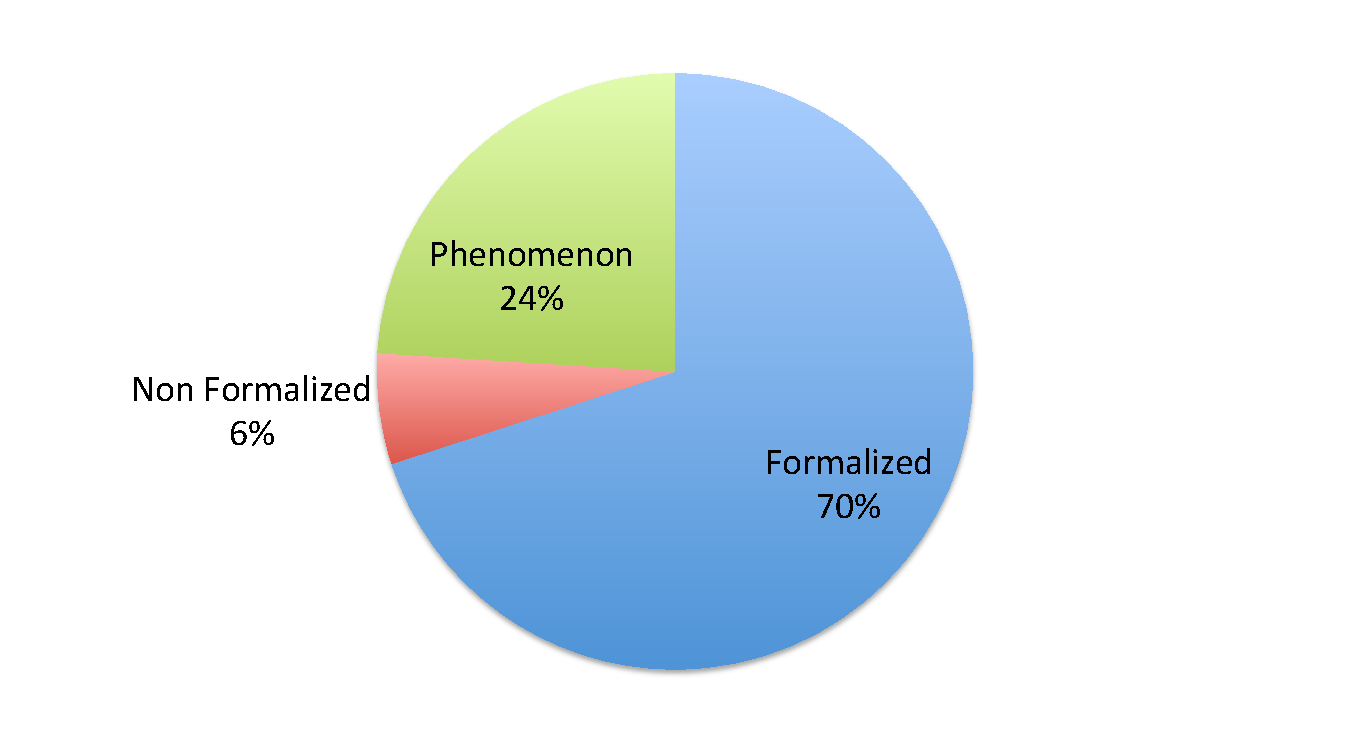
\includegraphics[width=0.47\textwidth]{main_formalization_results.pdf}
      \caption{\textbf{Figure \ref{fig:mainResults}:} Formalization results.}
      \label{fig:mainResults}
\end{figure}


\subsubsection*{\textbf{Formalized requirements}}
The second group of requirements includes the requirements that were successfully expressed with patterns. These requirements can be further divided into two big categories:
\begin{enumerate}
\item Requirements formalized without help of the engineers.
\item Requirements formalized with the help of the engineers.
\end{enumerate} 

The requirements falling into the first category typically looked like the following: 

\begin{enumerate}

\item \textit{``If lowFuelLevelWarningParam = 0, output lowFuelLevelWarning shall be set to Take No Action."}

\item \textit{``When DTC sensorShortToGround or sensorShortToBattery is set, the status of input signal fuelLevelSensor shall be set to ’Error’"}

\item \textit{``The CMS shall send a valid value in totalFuelLevel within 2 seconds from when the ECU starts."}\\
\end{enumerate}

In these examples, the behavior is clearly stated and the scope of the program execution can be identified, so the corresponding pattern can be found without requiring further assistance. We expressed the first two requirements with a \textit{Response} pattern, and the third one with a \textit{Bounded Response} pattern:
\begin{enumerate}
\item \textit{``Globally, it is always the case that if (lowFuelLevelWarningParam = 0) holds, then (lowFuelLevelWarning = 'Take No Action') eventually holds."}

\item \textit{``Globally, it is always the case that if (DTC sensorShortToGround or sensor ShortToBattery is set) holds, then (fuelLevelSensor = ’Error’) eventually holds."}

\item \textit{``Globally, it is always the case that if (ECU was started) holds, then (CMS sent valid signal to totalFuelLevel) holds after at most 2 seconds."}\\
\end{enumerate}

However, some of the requirements that could be formalized without engineers' assistance raised an interesting concern. It may happen that different patterns express semantics that are not easily distinguishable by a non-expert. This, combined with the inherent ambiguity of the natural language in which the requirements are written, may result in a wrong selection of a pattern; where wrong means ``not conveying the intention of the person writing the requirement". Such cases of incorrect disambiguation of requirements are particularly interesting because they may yield the results of the associated verification activities useless. As part of a larger process, the pattern selection should be validated by other means. However, analyzing the problem of validating the correctness of the pattern selection is out of the scope of this paper, and should be addressed only in a larger empirical case study with engineers taking part in the patterning process actively. In this work, a requirement is considered formalizable if there is at least one pattern that expresses the meaning of the requirement correctly as perceived by the researchers. For instance, let us consider the following requirement:

\begin{center}
\textit{``When parkingBrakeApplied has status 'Error' or 'Not Available' the replacement value 'Not Set' shall be used"}
\end{center}

To best of our knowledge, the semantics of the above requirement can be expressed with either \textit{Response} pattern with \textit{Global} scope or with an \textit{Universality} pattern with restricted scope \textit{After Q}. For clarification, we present the requirement expressed through both patterns, followed by their corresponding TCTL representation:
\begin{itemize}
\item \textit{``Globally, it is always the case that if (parkingBrakeApplied = 'Error' or parkingBrakeApplied = 'Not Available') holds, then (parkingBrakeApplied = 'Not Set') eventually holds."}

\item[] \vspace{0.1cm}
{\small
\begin{alltt}
AG[((parkingBrakeApplied = 'Error') OR 
(parkingBrakeApplied = 'Not Available')) \(\rightarrow\)
AF(parkingBrakeApplied = 'Not Set')]

\end{alltt}
}
\item \textit{``After ((parkingBrakeApplied = 'Error') or (parkingBrakeApplied = 'Not Available')), it is always the case that (parkingBrakeApplied = 'Not Set') holds."}
\item[] \vspace{0.1cm}
{\small
\begin{alltt}
AG[((parkingBrakeApplied = 'Error')
OR (parkingBrakeApplied = 'Not Available'))
\(\rightarrow\) AG(parkingBrakeApplied = 'Not Set')]

\end{alltt}
}
\end{itemize}

With the information given in the requirement alone, it is difficult to determine which of the patterns expresses the correct behavior to the full extend. The problem is that both patterns capture behaviors that are similar, but not equivalent, for instance because they are within different scopes. Potential causes of these problems are: the ambiguity of the requirement and the apparent overlapping between different patterns. The implications of choosing one pattern over the other are only evident in the following stages of the verification process, which are not considered in this case study.

Regarding the requirements for which assistance from the engineers was required, the most common difficulties were determining the scope of execution and understanding the underlying meaning. According to the Dwyer et al. \cite{Dwyer99sps}, there are five possible execution contexts for the patterns. Interestingly, none of them captures the moment of entering a particular state or executing a specific event. For example, let us consider the following requirement:
\begin{center}
\textit{``Output signal lowFuelLevelWarning shall have the initial value 'Not Active' at start-up."}
\end{center} 
This requirement imposes that the lowFuelLevelWarning signal shall receive some value when the system is \textbf{\textit{``in"}} some specific state (\textit{start-up}). None of the scopes capture the moment when the system is in a particular state but only \textit{Before} and \textit{After}, so we had to consult with the engineer in order to reformulate the requirement and expressed it with one of the defined scopes. For this particular requirement the \textit{After Q} scope was applied.

Another problem identified was that sometimes concepts from different level of abstractions were used, without specifying the meaning of the high level concepts. This problem may be related to the absence of phenomenon requirements that complement the semantics of the requirement, but it needs further investigation. For example, the following requirement is apparently well specified, but contains ambiguity:
\begin{center}
 \textit{``At the shut down, the last value of the totalFuelLevel shall be stored until next start-up."}
\end{center}

In this requirement, concepts from different levels of abstraction are present: the \textit{shut-down} and \textit{start-up} states/events belong to a higher abstraction level and are not properly specified, so their meaning is  ambiguous. More importantly, it is not clear what \textit{``the value"} is in this context and how and where it should be stored. For such requirements patterning is impossible unless an engineer disambiguate them.

\subsubsection*{\textbf{Non formalized requirements}}
The third type of requirements are the non formalized requirements. According to our experience, high complexity, high level of ambiguity and lack of information are the main reasons impeding the patterning of such requirements. We present one representative from this group:
\begin{center}
\textit{``Signal totalFuelLevel shall be output of a filter that includes information from both FLS\_vol and fuelRate to achieve a stable signal. The filter shall be implemented with a Kalman algorithm given by equations (2-4) with a feedback gain K."}\\
\end{center}

In this requirement, the relationship between the input and the output parameters has been defined with an analytical expression that is not present in the text. There is no approach that deals with transformation of analytical expressions into logic, so that the relationship between the input and the output parameters in this requirement cannot be formalized. For this reason, the requirement was classified as not formalizable. 

\subsection{Pattern frequency}

The distribution of the patterns used for formalizing the requirements in this case study is given in Figure \ref{fig:patternFreq}. Note that the distribution includes only the requirements formalized with patterns, and not the phenomenon requirements. From a total of seventeen patterns presented by Konrad and Cheng \cite{Konrad05sps}, seven were used in this case study. The distribution of the patterns is coherent with Post et al. \cite{Post12bosch} case study; this is an indication that a small number of patterns are enough to express the majority of the requirements in the automotive domain. The pattern most frequently used is  \textit{Precedence} followed by \textit{Universality}. It is interesting is that the \textit{Precedence chain 2-1} pattern was used in our case study, but not in Post et al's.

Another interesting difference between our results and the ones presented in the previous case study is the ratio between the \textit{Precedence} and the \textit{Response} patterns. In our case, most of the properties are expressed by using the \textit{Precedence} pattern, whereas Post et al's case study uses \textit{Response} pattern more often. These two patterns are very similar but not equivalent. This is due to the fact that the \textit{Response} allows effects to occur without causes, while the \textit{Precedence} allows causes to occur without effect. A number of factors can influence the application of both types of patterns, and we believe that the ambiguity of the requirements as well as the understanding of the underlying industrial systems are the most common ones. Our hypothesis is that within the verification phase, it will be possible to understand which one conveys better the requirement as originally intended by the engineer.

\begin{figure}
  \centering
    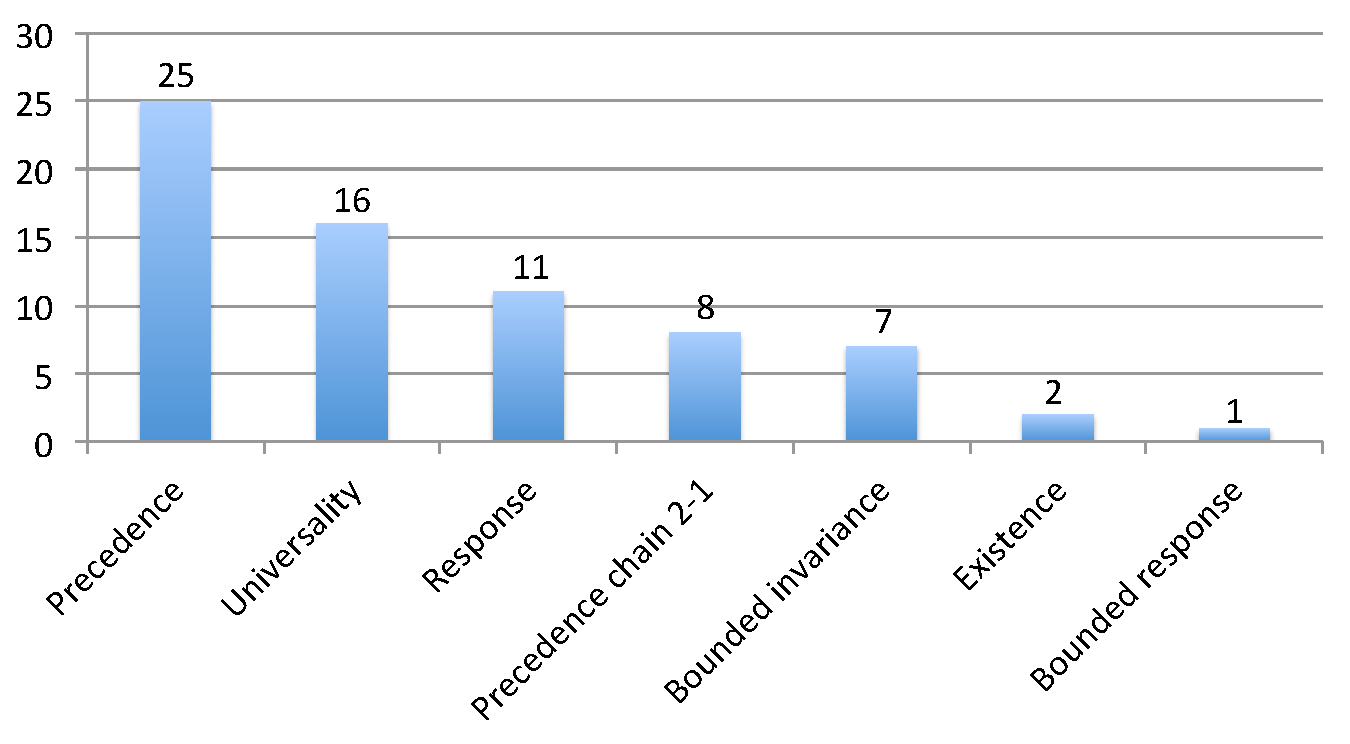
\includegraphics[width=0.47\textwidth]{pattern_ferquency_2.pdf}
      \caption{\textbf{Figure \ref{fig:patternFreq}:} Pattern frequency.}
      \label{fig:patternFreq}
\end{figure}


\section{Reflection on the experience}

According to our observations and expectations, the patterning process resulted into a number of benefits. One is an apparent reduction of ambiguity, due to the fact that the patterns tend to capture the \textit{``domain knowledge"} information, which is usually omitted in the requirements expressed in natural language. Additionally, in our conversations with the engineers, the patterns provided a useful support for discussing about the meaning of certain requirements. This is expected to impact positively on the communication between stakeholders, and also to improve testability of requirements.

The case study was completely focused on testing the expressiveness of the specification patterns on a functional requirements from the electrical and electronic systems installed in trucks. Driven by this specific goal, we did not take any precise measures about the effectiveness of the approach represented as patterning time per requirement. However, according to our observations, the patterning process was conducted in a reasonable time frame, thus making it applicable in industrial settings.

The case study also revealed certain limitations of the approach. Using patterns based on restricted English grammar eliminates the need to use mathematical expressions for formalizing the requirements, but the process still requires a significant effort. We observed that as the patterning process advanced, the researchers involved in the experiment became more proficient in using the patterns and also on the understanding of the requirements, which resulted in reducing the patterning time per requirement. 
But finding ways of softening this learning curve is desirable.

The main challenge of the patterning process is understanding the meaning of the patterns and the scopes of execution over which the patterns hold.
Post et al. \cite{Post12bosch} reported similar problems with respect to choosing the scope. Their experiment showed that the engineers favor the \textit{Global} scope because of its simplicity. According to them, this happens because the \textit{Global} scope captures the entire program execution, and thus it is easier to grasp.
Our case study, however, showed the opposite tendency. The researchers tend to understand the patterns better and have an inclination to use as much of the defined patterns and scopes as possible. Therefore, even though the extensive use of the \textit{Global} scope of execution can be accepted in most of the cases, finding more precise definition of the scope became a priority.

Although we believe that using restricted scopes is desirable, the implications of the effect from this decision is only visible in the next phases of the verification process. It remains as an open problem that will need further investigation.

\section{Conclusion}
This paper has discussed a case study intended to assess the suitability of using the specification patterns \cite{Konrad05sps} for formalizing E/E requirements in the automotive domain. The goal was to evaluate whether such patterns provide enough expressiveness and are, at the same time, easy to apply. Even though the case study was only a preliminary study of the problem, with some inherent limitations in size, a few interesting conclusions have been drawn.

The results of applying specification patterns to our set of requirements can be considered satisfactory. Among the  total set of requirements collected initially, 70\% were formalized with patterns. Considering only the behavioral requirements, 92\% of them were formalized. According to our observations, the patterning process reduced the ambiguity of the requirements and showed promising potential as a support to communication.

Our experience indicates that the patterns in their current form (a theoretical framework) are difficult to introduce in the industrial process. The patterns must be accompanied with support material, such as graphical representations and examples, which will make them more comprehensible for the engineers. Specifically, both the identification of patterns and the selection of scope of execution can be difficult sometimes, and may lead to wrong patterning; some extra information is needed to avoid this problem. In addition, providing user-friendly tool support will certainly favor industrial acceptance of the methodology and is most desired.

As a conclusion, the preliminary results showed that there is a strong need for conducting a more extensive case study including more engineers from different departments and more Scania E/E systems. To further increase the relevance of the results, we are also working towards including other companies from the automotive domain into the case study. In the new setup we expect to gain deeper understanding about the patterning process of the requirements, with a particular emphasis on identifying the engineers' needs. This data will be used for providing a tool to adequately support the process with a high level of correctness. However, even with an appropriate tool support, wrong interpretations may still happen in this initial phase, and the causes should be identified and investigated. When possible, these cases should be correlated to the engineers' background. 
The future case study will focus on accurately measuring the time required for patterning the requirements, in order to be able to draw statistical data such as formalization time per requirement. Additional effort is also needed for identifying the right metrics to study the quality of the requirements achieved through formalization as well as measuring (qualitatively) the engineers' perception about the benefits achieved through such formalization.

\section*{Acknowledgment}
This work was funded by the Swedish Governmental Agency for Innovation Systems (VINNOVA) under project 2013-01299.

%\section*{Acknowledgment}

\bibliographystyle{plainnat}

\begin{thebibliography}{1}

\bibitem{Alur92phd}
R.~Alur. \emph{Techniques for automatic verification of real-time systems.} PhD thesis, Stanford University, Stanford. 1992.

\bibitem{Cobleigh06userguide}
R. L. Cobleigh, G. S. Avrunin, and L. A. Clarke. \emph{User guidance for creating precise and accessible property specifications.} In Proc. of ACM SIGSOFT Found. on Soft. Eng. (FSE). 2006. pp. 208–-218.

\bibitem{Dwyer99sps}
M.~B.~Dwyer, G.~S.~Avrunin, J.~C.~Corbett. \emph{Patterns in property specifications for finite-state verification.} In Proceedings of the 21st international conference on Software engineering (ICSE '99). ACM, New York, NY, USA. 1999. pp.411--420. 

\bibitem{Hull11reBook}
M. Elizabeth, C. Hull, K. Jackson, J. Dick. \emph{Requirements Engineering, Third Edition.} Springer. 2011.

\bibitem{Emerson95temporaland}
E.~A.~Emerson. \emph{Temporal and modal logic}. In Handbook of Theoretical Computer Science. Amsterdam, Netherlands: Elsevier, 1995. pp. 995--1072.


\bibitem{Heumesser92experienceInAutomotive}
N.~Heumesser, F.~Houdek. \emph{Experiences in managing an automotive requirements engineering process.} In: RE, IEEE Computer Society. 2004. pp. 322--327.

\bibitem{Holberg11btc}
H. J. Holberg, U. Brockmeyer. \emph{ISO 26262 compliant verification of functional requirements in the model-based software development process.} White paper. Embedded World Exhibition and Conference. 2011.

\bibitem{iso26262}
International Organization for Standardization. \emph{ISO/DIS 26262-1 - Road vehicles — Functional safety.} International Organization for Standardization / Technical Committee 22 (ISO/TC 22). Geneva, Switzerland. 2009.

\bibitem{Konrad05facilitating}
S. Konrad and B. H. Cheng. \emph{Facilitating the construction of specification pattern-based properties}. In Proc. of the IEEE Int. Req. Eng. Conf. (RE). 2005. pp. 329–-338.

\bibitem{Konrad05sps}
S.~Konrad, B.~Cheng. \emph{Real-time specification patterns}. In Proceedings of 27th International Conference on Software Engineering. 15--21 May 2005. pp. 372--381.

\bibitem{Overmyer01conceptual}
S. P. Overmyer, B. Lavoie, and O. Rambow. \emph{Conceptual modeling through linguistic analysis using LIDA.} In Proc. of the IEEE Int. Conf. on Soft. Eng. (ICSE). 2001. pp. 401–-410.


\bibitem{Post12bosch}
A.~Post, I.~Menzel, J.~Hoenicke, A.~Podelski. \emph{Automotive behavioral requirements expressed in a specification pattern system: a case study at BOSCH.} In: Requirements Engineering Journal 17. March 2012. pp. 19--33.


\bibitem{Walia09sysLitReview}
GS.~Walia, J.C.~Carver. \emph{A systematic literature review to identify and classify software requirement errors.} Inf. Softw. Technol. 2009. pp. 51(7):1087–-1109.

\end{thebibliography}

% that's all folks
\end{document}


